\section{Blockchain-Assisted Assurance: Roles and Boundaries}

\subsection{The Decision to Use a Ledger}

The decision to use blockchain begins with the governance structure and required record semantics. A permissioned ledger is plausible when independently administered parties require joint control over accepted state transitions and cannot assign that role to one agreed custodian. Multi-party participation, signatures, or intermittent connectivity alone do not establish that need. A signed append-only log with independent witnesses, an authenticated database with protected audit records, or a jointly administered replicated database may provide the required accountability. The design should state which unilateral changes must be prevented, who can authorize conflicting updates, and which fault model the alternatives must tolerate before comparing their cost. Local verified control serves hard real-time loops.

A permissioned ledger is a plausible choice for the bounded-membership missions considered here because admission and endorsement can follow organizational authority. Permission model and consensus resource cost are separate design choices; permissionless participation does not necessarily imply proof of work. Resource-intensive peers and ordering services can reside on capable shore, edge, or selected USV nodes, while constrained vehicles submit transactions or verify supported proofs under explicit trust assumptions. Hyperledger Fabric provides a representative architecture with identities, endorsement policies, channels, ordering, and validation \citep{androulaki2018hyperledger,hyperledger2026fabric}. Its documentation distinguishes crash-fault-tolerant Raft ordering from Byzantine-fault-tolerant ordering. A Raft deployment does not obtain malicious-orderer tolerance merely from permissioned membership. Ordering, endorsement, and application validation protect different steps; clients must check a valid commit, since inclusion in a block need not mean a transaction updated application state \citep{hyperledger2026fabric}. OAL accommodates another shared-state service when its fault, availability, and governance assumptions match. Consensus surveys describe trade-offs among throughput, finality, membership, energy, and fault tolerance \citep{wang2019survey,lashkari2021comprehensive,zhang2020analysis}.

\begin{figure}[!htbp]
\centering
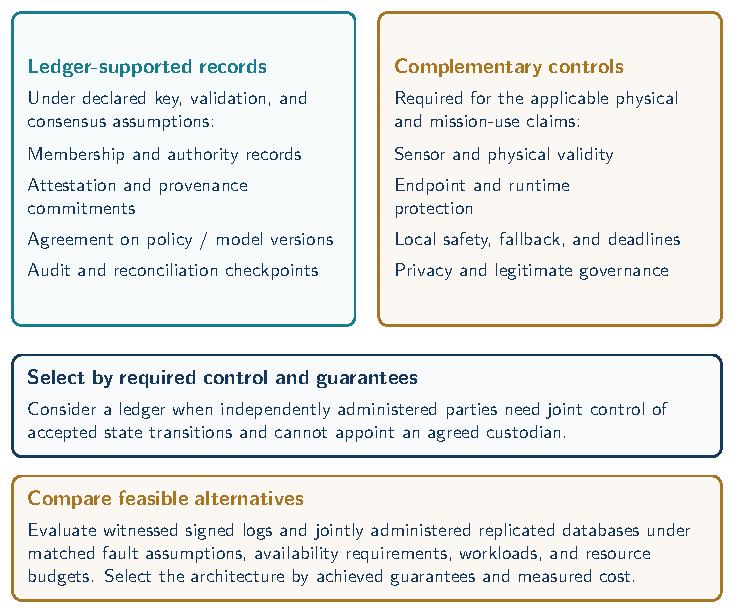
\includegraphics[width=0.92\textwidth]{figures/figure-06-blockchain-boundary.pdf}
\caption{Blockchain boundary in mission trust. Ledger-supported records and complementary controls serve distinct claims. Selection depends on required joint control and comparison with witnessed logs and replicated databases under matched assumptions.\label{fig:blockchain-boundary}}
\end{figure}

\subsection{On-Chain and Off-Chain Partitioning}

Raw video, sonar, point clouds, high-rate telemetry, detailed attestation evidence, and fine-grained location should remain off chain, encrypted and subject to data-use policy. The ledger records small, verifiable references: content identifiers or Merkle roots, producer and custodian identifiers, coarse timestamps or time ranges, schema and policy versions, attestation-result commitments, endorsement decisions, revocations, and audit outcomes. The commitment scheme specifies the exact bytes or canonical representation covered, its algorithm, and whether it commits to plaintext or ciphertext. Storage and retention arrangements preserve authorized access to the corresponding evidence; a digest supplies neither availability nor recoverability. The consumer records the ledger state, local authority information, and time uncertainty available at creation and use. Reconciliation separately evaluates these against subsequently learned events.

On-chain hashes provide integrity commitments. Privacy comes from encryption, access control, selective disclosure, retention rules, key destruction, aggregation, and metadata minimization, because hashes can reveal equality, support dictionary attacks on predictable values, and bind sensitive metadata to a durable member-visible record. On-chain metadata also persists after an off-chain object is deleted. Privacy design therefore accounts for traffic analysis, membership visibility, timing, and the linkage of vehicle identifiers across missions. General IoT and blockchain reviews identify privacy and storage tension \citep{reyna2018blockchain,li2020survey,nguyen2020blockchain}; maritime governance adds commercial and jurisdictional concerns \citep{li2021survey,farah2024survey,zhou2020key}.

\subsection{Five Design Patterns}

Table~\ref{tab:blockchain-patterns} organizes recurring ledger uses by OAL claim, assumptions, and complementary assurance requirements. The patterns synthesize UAV, IoT, provenance, and attestation work into reusable design templates.

\begin{table}[!htbp]
\caption{Blockchain design patterns for cross-domain mission assurance.\label{tab:blockchain-patterns}}
\begin{adjustwidth}{-\extralength}{0cm}
\scriptsize
\begin{tabularx}{\fulllength}{@{}P{30mm}P{35mm}P{40mm}YY@{}}
\toprule
\textbf{Pattern} & \textbf{On-chain record} & \textbf{Assurance supported} & \textbf{Necessary assumptions} & \textbf{Complementary assurance required}\\
\midrule
Membership and authority registry & Organization, role, credential status, delegation and revocation version & Cross-party identity and policy-state consistency & Governed issuer set, protected keys, bounded offline credentials & Real intent, endpoint integrity, emergency authority conflict\\
Attestation anchor & Evidence digest, verifier identity, result, reference-value and policy version & Accountable device-state appraisal and freshness history & Trustworthy measurement root and verifier; adequate coverage & Sensor truth, unmeasured runtime behavior, compromised verifier\\
Provenance commitment & Data/version identifier, transformation and custody roots, endorsement & Tamper evidence for recorded lineage and processing & Adequate instrumentation, bounded time uncertainty, protected keys, retrievable evidence & Semantic correctness, omitted events, biased models, metadata confidentiality\\
Partition-aware audit and reconciliation & Signed sequence range, batch root, local policy/model version, reconnect event & Detectable gaps or conflicts relative to retained checkpoints & Protected append state, independently retained checkpoints, eventual evidence retrieval & Unwitnessed suffix loss, uncaptured events, uncertain event time, physical truth\\
Policy/model coordination & Approved artifact identifier, activation/rollback time, authorized endorsers & Agreement on approved versions among synchronized participants & Governed approval, version validation, activation and rollback rules & Actual deployment state, partitioned participants, artifact safety and performance\\
\bottomrule
\end{tabularx}
\end{adjustwidth}
\end{table}

The membership pattern generalizes UAV identity and authentication proposals \citep{han2022identity,tan2022blockchain,karmakar2024blockchain}. It records which organization may issue each role, the applicable policy version, and how offline parties learn of revocation. Short-lived credentials, bounded delegation, and risk-specific offline envelopes constrain exposure while revocation information propagates.

Two full-text authentication studies provide prototype-level evidence for membership and channel establishment. Tan et al. evaluate Hyperledger Fabric smart-contract operations and cryptographic communication/computation costs in a simulated $10\,\mathrm{km}\times10\,\mathrm{km}$ UAV mission with cloud-hosted peers and assumed base-station coverage \citep{tan2022blockchain}. SwarmAuth combines PUF-based mutual authentication, a blockchain registry, and location-aware clustering, then evaluates security features, computation and communication cost, throughput, and delay using an EVM implementation and simulations \citep{karmakar2024blockchain}. OAL maps these results to entity/platform admission and ledger-supported registry claims. Observation validity, underwater partition behavior, cross-organizational governance, and consequence-weighted mission decisions form the corresponding cross-domain validation extensions.

The attestation pattern links RATS evidence appraisal to shared audit. An attester produces evidence; a verifier evaluates it under an appraisal policy; a relying party appraises the result for its intended use \citep{birkholz2023remote}. Recording a commitment to the result and policy supports later review and comparison of verifier outputs among organizations. Attestation architectures for blockchain and edge systems illustrate this intersection \citep{hardjono2021towards,ott2023universal,figueiredo2022arcadian,baciu2025secure}. Sensitive measurement detail remains encrypted off chain by default. The permitted age of a result is a relying-party policy bound, not a guarantee that device state remains unchanged until expiry; RATS explicitly recognizes the race between appraisal and subsequent state changes \citep{birkholz2023remote}.

Heterogeneous attestation is technically plausible, with platform-specific cost. The hardware-agnostic framework of \citet{ott2023universal} was implemented for TPM, AMD SEV-SNP, and ARM PSA evidence. Its mutual attested-TLS evaluation reported $31.2$ ms for SEV-SNP virtual machines on the same host and $476.1$ ms for the tested Intel firmware TPM, the latter dominated by quote generation. ARM PSA handshake latency was not measured because TLS was not implemented on that embedded device. These configuration-specific results are not a cross-domain communication benchmark. They motivate retaining technology, configuration, freshness, and measurement scope with an attestation result. Measured software identity must also be interpreted against reference values and software assurance evidence; matching an approved image does not demonstrate that it is vulnerability-free or that its sensor observations are accurate.

The provenance pattern links W3C-compatible derivation to shared commitments. IoT provenance proposals use blockchain to protect provenance records or bind large off-chain collections \citep{hang2019design,honarpajooh2021iot,khan2020iot,rahman2020secure}. For mission data, each derived product should identify immutable inputs, transformation code or model, parameters, responsible entity, and output version. Provenance supports explanation and accountability, including for AI artifacts \citep{kale2023provenance}; observation-validity and mission-suitability appraisal assess the semantic quality of the transformation and its output.

The partition-aware pattern is especially relevant to underwater missions. A node or gateway keeps a signed, hash-linked local sequence, retains a batch root locally during disconnection, and submits it with a sequence range and prior checkpoint when connectivity permits. Verifiers check signatures, membership evidence, sequence continuity, duplicates, policy versions, and consistency with independently retained checkpoints. Inclusion proofs establish membership in a committed batch; they do not establish that every physical event was captured. Missing entries inside a known sequence range or conflicting disclosed histories may be detected, while deletion of an unwitnessed suffix can remain invisible. Protected counters, independently held receipts, and explicit capture assumptions determine the strength of the audit claim.

Partition handling separately specifies ledger safety, ledger liveness, and local mission authority. Here, ledger safety means that correct replicas do not finalize conflicting histories under the selected protocol's assumptions; liveness means that eligible requests can progress when its quorum and communication conditions hold. Losing the required quorum can suspend new commits while previously verified records remain locally usable. The CAP result concerns the impossibility of simultaneously guaranteeing linearizable shared read/write state and completion of every request at nonfailed nodes under arbitrary partitions \citep{brewer2000towards,gilbert2002brewer}. It does not require every local mission function to stop or guarantee a real-time deadline. Predelegated local actions can continue within their envelope, but an offline decision that requires fresh global state must wait, use an explicitly weaker state assumption, or follow its authorized fallback. Later reconciliation records conflicts and their disposition; it cannot retroactively make an unsafe physical action safe.

\subsection{Governance, Revocation, and Recovery}

Permissioned consensus places trust in explicit consortium rules. A consortium defines member eligibility, validator distribution, endorsement thresholds, emergency powers, software upgrade, key rotation, data jurisdiction, dispute resolution, incident disclosure, and exit. Multiple replicas controlled by one administrator do not provide independent organizational control of history. Conversely, different organizational names do not establish fault independence if validators share administrators, cloud credentials, software defects, or key custody. The governance assessment therefore identifies who can change membership and policies, override controls, or deny a quorum. Endorsement thresholds and validator placement must be evaluated against that distribution of authority and the required availability.

Revocation is temporal. A credential revoked with effect from 12:00 may have authorized a disconnected UUV's action at 11:55, while the gateway learns the revocation at 12:30. This interpretation requires a declared effective-time rule and trustworthy bounds on the action time; a signed timestamp alone cannot establish when the event occurred. Audit separates event-time intervals, receipt and commitment times, locally known credential status, the applicable delegation, and subsequently learned revocation. If the event-time interval overlaps revocation or key compromise is suspected, the validity finding may remain disputed. Recovery reviews identities, affected models, data products, recorded provenance descendants, device re-attestation, and consequential mission decisions. The ledger and dependency graph help locate the recorded affected set; missing lineage requires additional investigation.

\subsection{Real-Time and Safety Boundaries}

Deadline-bound vehicle functions require local control with timing and safety arguments appropriate to stabilization, collision avoidance, or an emergency maneuver. The ledger can coordinate approved policy or software versions before operation, record summaries afterward, and support slower supervisory decisions, cross-party authorization, data release, and audit. Removing a ledger dependency from a control path avoids making consensus progress a prerequisite for that path, but platform safety still depends on local sensing, control, resources, and the chosen fallback. For example, emergency surfacing must itself be assessed against the local environment. Reduced audit freshness and cross-organizational coordination remain visible during ledger-service loss.

Figure~\ref{fig:blockchain-boundary} provides a claim discipline. Under the configured fault and key assumptions, a ledger supports evidence about accepted endorsements, versions, and record order. Physical, endpoint, timing, privacy, and governance evidence is additionally required to assess whether observations matched the world, endpoints met their integrity requirements, deadlines were satisfied, and authority was appropriate.
